\documentclass[11pt,a4paper]{report}


%%% packages

  \usepackage{a4wide}           % set page size etc
  \usepackage{graphicx}  
  \usepackage{epstopdf}         % to include figures in .eps-format
  \usepackage{multido}          % used in chapter 3 to repeat text
  \usepackage{setspace}         % provides \onehalfspacing
  \usepackage{url}              % to set URLs, paths, commands ... in tt
  \usepackage{amstext}          % provides \text, which, unlike \mbox, scales
  \usepackage{amsmath}          % provides align and align*, besides others
% \usepackage{times}            % switches to the Times font, saves space
  \usepackage{amssymb,mathptmx} % provides more math symbols
  \usepackage{hyperref}
  \usepackage{algorithm}
  \usepackage{algorithmic}
  \usepackage{svg}
  \usepackage{tikz}
  \usepackage{listings}
  \usepackage{booktabs}
  \usepackage{pgfgantt}
  \usepackage{todonotes}

  \DeclareGraphicsExtensions{.eps}
  \DeclareGraphicsExtensions{.png}

  \usetikzlibrary{positioning}
  \usetikzlibrary{fit}
  \tikzstyle{line}=[draw]
  \tikzstyle{arrow}=[draw, -latex] 
%%% new commands
  
  \newcommand{\PD}[2]{\frac{\partial #1}{\partial #2}} % partial derivation
  \newcommand{\dd}{\,\mathrm{d}} % to be used in differentials

  \newcommand{\nocontentsline}[3]{}
  \newcommand{\tocless}[2]{\bgroup\let\addcontentsline=\nocontentsline#1{#2}\egroup}

% Rules for handling pre-zipped figures. To create zipped figs do this:
% $ head myfigure.eps > myfigure.eps.bb
% $ gzip myfigure.eps
  \DeclareGraphicsRule{.eps.gz}{eps}{.eps.bb}{`zcat #1}
  \DeclareGraphicsRule{.epsi.gz}{eps}{.epsi.bb}{`zcat #1}
  \DeclareGraphicsRule{.eps.Z}{eps}{.eps.bb}{`zcat #1}

%%% One and a half line spacing

% \renewcommand{\baselinestretch}{1.5}
  \onehalfspacing % better than \renewcommand{\baselinestretch}{1.5}


%%% other styles

  \setcounter{secnumdepth}{3}
  \setcounter{tocdepth}{4}

%%% Set citations and toc as links
  \hypersetup{
    colorlinks,
    citecolor=black,
    filecolor=black,
    linkcolor=black,
    urlcolor=black
  }

\makeatletter
\pgfdeclareshape{document}{
\inheritsavedanchors[from=rectangle] % this is nearly a rectangle
\inheritanchorborder[from=rectangle]
\inheritanchor[from=rectangle]{center}
\inheritanchor[from=rectangle]{north}
\inheritanchor[from=rectangle]{south}
\inheritanchor[from=rectangle]{west}
\inheritanchor[from=rectangle]{east}
% ... and possibly more
\backgroundpath{% this is new
% store lower right in xa/ya and upper right in xb/yb
\southwest \pgf@xa=\pgf@x \pgf@ya=\pgf@y
\northeast \pgf@xb=\pgf@x \pgf@yb=\pgf@y
% compute corner of ‘‘flipped page’’
\pgf@xc=\pgf@xb \advance\pgf@xc by-10pt % this should be a parameter
\pgf@yc=\pgf@yb \advance\pgf@yc by-10pt
% construct main path
\pgfpathmoveto{\pgfpoint{\pgf@xa}{\pgf@ya}}
\pgfpathlineto{\pgfpoint{\pgf@xa}{\pgf@yb}}
\pgfpathlineto{\pgfpoint{\pgf@xc}{\pgf@yb}}
\pgfpathlineto{\pgfpoint{\pgf@xb}{\pgf@yc}}
\pgfpathlineto{\pgfpoint{\pgf@xb}{\pgf@ya}}
\pgfpathclose
% add little corner
\pgfpathmoveto{\pgfpoint{\pgf@xc}{\pgf@yb}}
\pgfpathlineto{\pgfpoint{\pgf@xc}{\pgf@yc}}
\pgfpathlineto{\pgfpoint{\pgf@xb}{\pgf@yc}}
\pgfpathlineto{\pgfpoint{\pgf@xc}{\pgf@yc}}
}
}
\makeatother

\usepackage{microtype}

% Scala Listings support
\lstdefinelanguage{scala}{
  morekeywords={abstract,case,catch,class,def,%
    do,else,extends,false,final,finally,%
    for,if,implicit,import,match,mixin,%
    new,null,object,override,package,%
    private,protected,requires,return,sealed,%
    super,this,throw,trait,true,try,%
    type,val,var,while,with,yield},
  otherkeywords={=>,<-,<\%,<:,>:,\#,@},
  sensitive=true,
  morecomment=[l]{//},
  morecomment=[n]{/*}{*/},
  morestring=[b]",
  morestring=[b]',
  morestring=[b]"""
}

\begin{document}

\tikzstyle{doc}=[%
draw,
thick,
align=center,
color=black,
shape=document,
minimum width=20mm,
minimum height=28.2mm,
shape=document,
inner sep=2ex,
]

\thispagestyle{empty}

\vspace*{73.5mm}
\begin{center}
  \setlength{\unitlength}{1mm}
  \begin{picture}(110,60)
    \put(-1,0){\makebox(110,60){% 1mm off the centre to match the hole
        \begin{minipage}{110mm}%% in the lime green card board cover
          \begin{center} \Large
            \textbf{Efficient Parallel Data Processing \\ in the Cloud} \\
            {Ashley Ingram} \\
            {BSc Computer Science} \\
            {2013/2014}             
          \end{center}
        \end{minipage}
      }}
    \put(54,30){\oval(110,60)}% 1mm off the centre too
  \end{picture}
\end{center}
\vspace*{\fill}

\noindent 
The candidate confirms that the work submitted is their own and the
appropriate credit has been given where reference has been made to the
work of others.

\quad

\noindent 
I understand that failure to attribute material which is obtained from 
another source may be considered as plagiarism.

\quad

\begin{flushright}
  (Signature of student)\underline{\hspace*{2in}}
\end{flushright}

          % This is the front page

\pagestyle{plain}        
\pagenumbering{roman}    % Set up page numbering
\setcounter{page}{1}

\begin{center}
    {\LARGE\bf Summary}
\end{center}

Fill in the summary here.

        % Summary
\begin{center}
    {\LARGE\bf Acknowledgements}
\end{center}

Most of all I'd like to thank my project supervisor \dots

% \newpage

    % Acknowledgements
\tableofcontents
\newpage

\pagenumbering{arabic}   % Set up page numbering
\setcounter{page}{1}

\chapter{Introduction}
\label{CHAP_FIRST}
\centerline{\rule{149mm}{.02in}}
\vspace{2cm}
\section{Project Aim}
Large scale data processing is an emerging trend in Computing, with benefits to both academia and industry. The aim of this project is to investigate the challenges of large scale parallel data processing, discuss the benefits of Cloud Computing and investigate how the efficiency of large scale data processing may be improved. 

This project will aim to provide a reasoned and objective evaluation of the efficiency of data processing techniques, whilst comparing current state of the art tools and technologies with newer research in the field. 

Specifically, the data processing tools Hadoop and Nephele will be compared, allowing comparison of the individual tools, and a wider discussion of the pros and cons of the MapReduce and PACT programming paradigms. 

\subsection{Research Questions}
The project aims to answer the following questions:

\begin{itemize}
	\item Does PACT overcome the inherent disadvantages of the MapReduce paradigm?
	\item How well does Nephele perform MapReduce tasks?
	\item How do Hadoop and Nephele perform in a highly elastic Cloud Computing environment?
\end{itemize}  

\section{Objectives}
The objectives of the project are:

\begin{itemize}
	\item Investigate Cloud Computing, Big Data and other relevant background trends
	\item Design a series of experiments to determine the efficiency of data processing technologies
	\item Implement the experiments for both Hadoop and Nephele
	\item Evaluate the experiment results to draw meaningful conclusions to the research questions
\end{itemize}

\section{Methodology}
The project will be broken into three main phases. The order to the phases provides a structured approach to the project, and completion of each phase ensures the project is completed in a methodical manner. The \textbf{Background Research} section will provide a comprehensive literature review to provide context to the project. This will be followed by a phase of \textbf{Experimentation}, which will aim to test the necessary factors of Hadoop and Nephele to answer the research questions. Finally, the \textbf{Evaluation} phase will evaluate the results of the experiments and the project as a whole.

The phases of the project will be performed according to Agile principles. Work will be carried out in weekly sprints, with clearly defined targets for each sprint. Supervisor meetings will be used as an opportunity to reflect on the achievements and shortcomings of the previous week, and to set targets for the upcoming sprint.

\subsection{Background Research}
The background research will aim to provide context for the project by surveying the current research landscape. It will summarise the fundamental concepts underlying the project and give a strong theoretical foundation for the rest of the project.

The first section of the background research will focus on Cloud Computing. It will explore the principles of the cloud, the service and deployment models and the technologies which make the cloud possible. It will also look at the unique advantages that the cloud provides in data processing scenarios.

The second segment of the background research will look in to Big Data and what challenges it introduces. An overview will be given of tools and techniques which have been developed to process Big Data, including Hadoop and Nephele.

\subsection{Experimentation}
Experiments will be designed to test the efficiency of data processing tools in relevant situations. This will require identifying relevant areas of interest, and deriving scenarios which will test the efficiency of Hadoop and Nephele. The experiments should be designed to take into account the various different problems that data processing tools are required to solve and to provide findings for the research questions.

As part of the experiment design, a hypothesis will be produced.

The experiments will be implemented and executed, in order to provide results which can be used to answer the research questions.

\subsection{Evaluation}
The project can be evaluated on various factors.

A technical evaluation will be carried out to analyse the results of the experiments. It will compare the efficiency of Hadoop and Nephele, referring to data obtained in the experimentation phase. The results will be compared to existing research (obtained during the background research) and the hypothesis, and any discrepancies will be discussed. 

An evaluation will also be carried out to determine whether the aims and objectives of the project have been met. This will involve determining whether the research questions have been answered in a satisfactory manner, and determining the relevance of the project in regards to existing literature and how it contributes to the research landscape. Any future scope for research will be identified. 

The methodology and management of the project will also be evaluated to identify areas of improvement in project management. This evaluation will be carried out in the personal reflection.

\section{Schedule}
The project schedule will be created around a set of fixed milestones in the project process. Work will be allocated in weekly sprints to ensure that the relevant work is completed in time for each milestone. Work will be prioritised so that scope can be cut to meet a milestone if required.

\subsection{Milestones}
There are a series of milestones which must be met throughout the project. This provides a framework for the project plan, as necessary tasks must be completed before the milestones.

\begin{enumerate}
	\item Submission of Aims \& Objectives

	The Aims \& Objectives of the project must be decided, which is crucial in setting the scope and direction for the rest of the project.

	\item Presentation to the Distributed Systems and Services Group

	The presentation to the Distributed Systems and Services group provides an opportunity to get early feedback on the project, and present much of what will be present in the mid year report. In order to present the project, a sufficient amount of content must be prepared. By this point a substantial amount of background research should have been carried out, and early ideas about experimental design should be formed.

	\item Mid-Year Project Report

	The Mid-Year Project Report is a chance to get feedback from the assessor about the direction and progress of the project. By this stage the background research should be completed, and should demonstrate that necessary steps have been taken to understand the problem. The Aims \& Objectives should be clearly defined, with a set of deliverables, a methodology, and a schedule. At this point experimental design will not have been completed, but the Mid-Year Report should give indications about the type of experiments that will be executed and why they were chosen. Finally, evidence of basic implementation should be shown, to demonstrate knowledge of the tools required for experiment implementation. 

	\item Progress Meeting

	The progress meeting occurs in the late stages of the project, so at this point most of the work should be completed. Experiments should have been implemented and performed, and code should be available for inspection.

	\item Final Report Submission
	
	The final report submission marks a point where all work on the project has to be complete. 
\end{enumerate}

\section{Deliverables}
The project will deliver 2 things.

\begin{enumerate}
	\item An evaluation of the efficiency of Hadoop and Nephele in various data processing situations
	\item Code for experiments, designed to test the efficiency of Hadoop and Nephele
\end{enumerate}       % include the chapters
\chapter{Background Research}
\label{CHAP_SECOND}
\centerline{\rule{149mm}{.02in}}
\vspace{2cm}
This chapter is intended to give an overview of the current research landscape, and to summarise the core technologies and concepts which form a basis for this project. The chapter will discuss trends toward Cloud Computing, how it is relevant to Data Processing, and key technologies which have been developed in this area, giving a foundation for further investigation into the efficiency of Data Processing techniques and how they are impacted by the Cloud. 

\section{Cloud Computing}
Cloud Computing is the latest major infrastructure paradigm which looks to deliver on the promise of Utility Computing. In practice, the term `Cloud Computing' is ambiguous. Whilst no clear definition exists many experts agree that the cloud exhibits the core benefits of Utility Computing such as elasticity and scalability, whilst making heavy use of virtualisation and pay-per-usage business models \cite{vaquero2008}.

Elasticity in clouds refers to the ability for a user to dynamically select the amount of computing resources they require, allowing them to scale their applications according to demand. The resources that can be acquired are essentially limitless from the user's perspective. \cite{mell2011nist} 

Elasticity represents a dramatic shift from the `traditional' method of building and deploying applications. Rather than purchasing and provisioning hardware and acquiring physical space (such as a data centre), a user can use a Cloud Service Provider. This allows for greater flexibility in business and application development, as users can cope with unpredictable or inconsistent levels of demand. An example of where this flexibility would benefit a company is in the case of an online store. A store may receive fluctuating traffic throughout a year, such as being particularly busy around the Christmas period. It would be economically inefficient for the store to purchase extra servers to cope with demand over the festive period, as they would be redundant for the majority of the year, but they must improve hardware capability in order to take advantage of the extra business. The inherent flexibility from the elasticity of the cloud would allow the store to simply acquire new computing capacity from their Cloud Service Provider on a temporary basis, giving them the capability of accommodating with the peak traffic but not using (or paying for) the extra resources when they are not needed. Having this scalability is seen as a core benefit of Cloud Computing.

A Cloud Service Provider is an organisation that provides access to Cloud Computing resources. They manage the underlying hardware, and typically provide APIs and other methods for a user to manage their resources. Some of the largest Cloud Service Providers are Amazon through AWS (Amazon Web Services), Microsoft through Windows Azure and Google through Google Apps.

A Cloud Service Provider does not have to be an external organisation, but when they are they typically use pay-per-usage business models. Rather than pay a fixed monthly cost, or have a one-off license fee, customers will pay the Cloud Service Provider for the resources they use (usually on a per-hour basis). For example, a `Medium' size Virtual Machine costs £0.077 an hour from Windows Azure \cite{AzurePricing}. This allows businesses to only pay for the resources that they need.

\subsection{Related Ideas}
\subsubsection{Utility Computing}
Utility Computing is the idea that households and businesses could outsource their demand to external companies, who provide the relevant amount of service on a pay-per-usage basis. Customers would access computing resources over a network, and would pay for the length of computing time that they use.

This is analogous to other utilities such as Gas or Electricity. In the case of Electricity, power is provided from the National Grid and the customer pays for how much they use. This allows a customer change the amount of power they require without having to pay a fixed cost (for example, using less electricity when they are on holiday).

Utility Computing is an established concept, with leading thinkers such as Leonard Klienrock (part of the original ARPANET project) referencing it as early as 1969 \cite{319}. Various technologies have emerged which offer some attributes associated with utility computing, with Grids and Clouds appearing to be the most promising \cite{buyya2008market}.

\subsubsection{Virtualisation}

\section{Cloud Computing Service Models}
Depending on the scenario, the Cloud offers several different service models. These models allow for clients to provision services in a different manner, depending on what they need from the cloud.

The different service models provide different levels of abstraction for the user. In Infrastructure as a Service, the user has full control over the machines that they acquire from the Cloud Service Provider, where in Software as a Service they are given less control, and need not worry about the underlying hardware whatsoever.

\subsection{Infrastructure as a Service}
Infrastructure as a Service (IaaS) provides an abstraction on top of a virtualisation platform, so that the client does not need to worry about what method of virtualisation is being used, and does not have to learn about the underlying technologies \cite{amies2012}.

Clients can request Virtual Machines in varying configurations, and a Virtual Infrastructure Manager will provision an appropriate Virtual Machine on a physical machine which has capacity. In addition to allowing users to provision virtual machines, IaaS systems may allow a user to configure other infrastructure elements, such as virtual networks. 

This provides a great deal of control to the user, as they are essentially renting a machine of a requested specification for a short period of time. They are free to install whatever Operating System and software on the machine as required, and can configure it in essentially any way. 

An example of an Infrastructure as a Service provider would be Amazon EC2 \cite{amazonEC2}. Amazon provide a variety of different Virtual Machine types, including those specialising in High Performance Computing or applications requiring a large amount of memory. Virtual Machines can use a range of images provided by Amazon (including Windows and various distributions of Linux), or users can create and upload their own custom Virtual Machine images. 

\subsection{Platform as a Service}
Platform as a Service (PaaS) is a higher level abstraction which allows applications to be built and deployed without worrying about the underlying Operating System or runtime environment \cite{intelPaaS}. The user still specifies the resources required, but no longer has to manually manage the virtual machines. The Cloud Service Provider will maintain the machines, providing the necessary software (Operating Systems, Web Servers, etc) and updating them frequently.

The advantage of PaaS is that it allows users to deploy their own applications, without having to worry about maintaining the underlying infrastructure. Whilst this decreases the control the user has over the deployment environment, it reduces the complexity of managing the infrastructure themselves. 

PaaS offerings may also provide supplementary services to users, such as health and availability monitoring, or auto-scaling.

Windows Azure is an example of a Platform as a Service provider \cite{azure}. Whilst they provide Infrastructure as a Service offerings, they also provide Platform as a Service capabilities through Windows Azure Web Sites. Windows Azure Web Sites allow users to upload applications written in a variety of web technologies (ASP.NET, Python, PHP, Node.js) and have them hosted in the Windows Azure runtime environment. This means the client does not manually have to manage web servers, frameworks and other necessary technologies.

\subsection{Software as a Service}
Software as a Service (SaaS) refers to providing access to applications over the internet on-demand \cite{zhang2010cloud}. Software is centrally hosted by the Cloud Service Provider, and clients can access the application through a web browser or other form of client. As the software is centrally hosted, Cloud Service Providers can handle updating the software for all users, ensuring all users benefit from bug fixes or additional features. 

Software as a Service applications can reduce the cost of deploying and using software for an organisation as they don't have to purchase their own hardware, install and configure software, and can avoid having technical support staff. An example of a successful Software as a Service application is Salesforce \cite{salesforce}. Salesforce is a Customer Relationship Management tool which charges organisations per user, making it a viable choice for small businesses. Salesforce can be accessed through a web browser, enabling customers to use their software regardless of location or device. 

\section{Cloud Computing Deployment Models}

\section{Big Data}

\section{MapReduce}

\section{PACT}

\section{Summary}
\chapter{Experiment Design}
A series of experiments have been designed in order to objectively analyse the efficiency of Stratosphere and Hadoop. This section discusses the design of the experiments in regards to the aims of the project.

Experiments are designed in a modular fashion, enabling a subset of them to be completed whilst still providing relevant research results. This approach was taken to limit the risk that is introduced by the time constraints of the project. 

\section{Experiment Variables}
There are a total of 30 experiments with 3 varying factors, in order to test the data processing tools in a range of relevant scenarios. 

\subsection{Data Processing Tools}
The first factor that will be varied is the tool used to process the data. This relates to the first two research goals: providing a comparison of the MapReduce and PACT programming paradigms, and ascertaining how well Stratosphere can perform MapReduce tasks.

\subsubsection{Hadoop}
Hadoop is an open source implementation of the MapReduce paradigm, which has become the de-facto standard for big data processing \cite{qin2013reflection}. This makes it an ideal choice for comparing MapReduce and PACT.

Experiments will be run in Hadoop to provide an indication of the efficiency for the current state of the art in data processing. This provides a reference point to which alternative data processing technologies can be compared. 

\subsubsection{Stratosphere (PACT)}
Stratosphere is a tool which implements the PACT programming paradigm, which as a superset of MapReduce can also perform tasks in a MapReduce style. This means that experiments can be implemented using the same tool, but in different programming paradigms, allowing a fair test of PACT vs MapReduce. This is designed to answer the first research question, namely whether or not PACT overcomes the inherent disadvantages of the MapReduce paradigm.

In a broader sense, it allows a complete comparison of Hadoop and Stratosphere. In real-world data processing scenarios, users of Stratosphere would be unlikely to restrict their programming options to just MapReduce, and would be likely to use other aspects of PACT as appropriate. Running experiments in the same way allows a fairer comparison of the 2 tools, where all of their functionality is available.

\subsubsection{Stratosphere (MapReduce)}
Experiments will also be run using just the Map and Reduce operations of Stratosphere. Whilst Stratosphere has a wider set of operations, solving data processing tasks using just Map and Reduce allows Stratosphere and Hadoop to be directly compared, aiming to answer the second research question. If Stratosphere can perform MapReduce tasks with comparable efficiency to Hadoop, it will indicate that Stratosphere is a more efficient tool for large-scale data processing in general, not just for those situations where a problem cannot be formulated in terms of MapReduce.

\subsection{Data Processing Task}
The second varying factor will be the data processing task that the tools have to complete. The tasks have been chosen to represent real-world issues as closely as possible, to give an indication of performance in scenarios where the tools are likely to be used, rather than having synthetic benchmarks such as word counting or Terasort. 

\subsubsection{Reverse Link Graph}
The first problem the data processing tools will have to solve is generating a Reverse Link Graph \cite{dean2008mapreduce}. In some situations, finding the transpose of a directed graph can be difficult. For example, when considering the Web Graph; it is relatively trivial to find the edges coming out of a vertex (as the hyperlinks on a page indicate its outgoing edges), but it is far more difficult to find incoming edges (pages which link to the current page). 

The Reverse Link Graph problem has been solved as it is a `classic' MapReduce problem. A `classic' MapReduce problem is a problem which can easily be formulated in terms of MapReduce. Classic MapReduce problems tend to be stateless, and do not depend on other parts of the data. This makes it easier to compute the solution in parallel, but means that many problems are not well suited to MapReduce (such as naturally iterative problems). An example of a classic MapReduce problem would be Word Counting, as each document can be processed in parallel. 

The Reverse Link Graph has been chosen in order to measure how effective both Hadoop and Stratosphere are at processing data using the MapReduce paradigm. This specifically relates to the second research question (``How well does Stratosphere perform MapReduce tasks?'').

Finding a reverse link graph of the web is a key component in many search engines \cite{page1999pagerank} where backlinks are used to indicate how important a page is, and can also be used to analyse a network of academic articles by treating references as edges \cite{garfield2002algorithmic}. 

\subsubsection{PageRank}
The second problem for the data processing tools to tackle is the PageRank algorithm. PageRank is a method of objectively and mechanically rating the importance of a web page, trying to measure human interest and the attention paid to the page \cite{page1999pagerank}. 

The PageRank algorithm is an example of the type of problem that MapReduce is traditionally cited as being poor at completing. It is an iterative algorithm which converges on a PageRank for each node. It requires information from adjacent nodes to compute a nodes PageRank at each step, which means that each step of the iteration must be performed sequentially, as part of a separate MapReduce pass.

By contrast, PageRank should use many of the additional features that the PACT programming model provides over MapReduce. The presence of iteration support and dedicated operations for Joins should test the additional operations that PACT provides in order to determine whether they yield tangible performance benefits.

Computing the PageRank of a graph of pages is a suitable test of how well the PACT programming model overcomes the issues of MapReduce, as it exercises many of the additional features. This will provide an answer to the first research question (``Does PACT overcome the inherent disadvantages of the MapReduce paradigm?'').

\subsection{Cluster Size}
The size of the cluster will be varied in order to give an indication of how well the data processing technologies perform at scale. This is a key factor in processing large scale data, as technologies which do not scale well as machines are added are unlikely to perform well in real-world scenarios, where the size of data may run into the Petabytes.

The elasticity of the Cloud will be required to scale the size of the cluster for different experiments. Specifically, experiments will be run using 2, 4, 6, 8 and 10 nodes. Scaling the size of the cluster will test both the scalability of the data processing tools, and the ability for the tools to harness the elasticity of the cloud, meeting the third research aim.

\section{Measurements}
Measurements will be taken from the experiments in order to give quantitative metrics which can be used for objective analysis.  

\subsection{Runtime}
Runtime is the length of time that a program (or data processing task) takes to execute. Runtime is one of the primary mechanisms for determining the efficiency of the data processing solutions. The time it takes to perform a task is a key element in large scale data processing, as the sheer scale of data can cause operations to take a long period of time. 

\subsection{Scalability}
The Scalability of data processing tools is also a key metric in determining how efficient they are. The scalability of a system refers to how well it accommodates additional resources \cite{bondi2000characteristics}, such as additional machines. 

In the context of Data Processing tools such as Hadoop and Stratosphere, it is desirable for systems to be able to scale according to both the size of data, and the number of nodes in the cluster. A data processing tool should be able to handle any amount of data, providing that it has the correct amount of system resources. Indeed, this is what distinguishes tools like Hadoop from other data processing tools such as numpy - the ability to analyse petabytes of data. A Data Processing system should also be able to scale according to the number of nodes added. There should be no upper limit to the number of nodes in a cluster, as this provides an important mechanism of adding the necessary resources to handle larger processing tasks. Adding a large number of nodes with lesser resources may be more cost efficient than adding fewer nodes which have comparatively larger system resources. This may be a reason why many users that engage in large scale data processing build clusters from commodity components \cite{taylor2010overview}.  

% TODO: Is the derivative acceptable?
The specific type of scalability that will be considered in these experiments is Runtime Scalability. Intuitively, as nodes are added to the cluster the runtime for experiments should decrease as work can be partitioned out to a larger set of working nodes. In an ideal world, this would follow a linear progression; as the number of processors is doubled the runtime should be halved. This can be measured by taking the runtime of a task when the processor count doubles (so the processor count is $2^{p}$ where $p$ is an integer representing the processor count) and taking the derivative. 

\subsection{Alternative Measurements}
Various alternative mechanisms could be used to determine the efficiency of the data processing tools. The scope of the project will be limited to measuring the runtime and runtime scalability, but some other measurements which could be used are as follows.

\subsubsection{Data Scalability}
It is important for clusters to be able to deal with large amounts of data in a reasonably efficient manner. A further test of scalability would be to test the cluster with various different datasets of different sizes. As with runtime scalability, this would ideally be linear, so that when the size of the data is doubled, runtime would also approximately double. The data processing tools may be of less use if the runtime increase is larger (for example, an exponential increase in runtime) as this would make running tasks on petabytes of data unreasonable.

\subsubsection{Resource Utilisation}
The resources used on nodes can be measured to determine how efficient the data processing tool is. An efficient data processing tool could be defined as one which uses the resources of each node effectively, by utilising a high amount of memory and CPU capacity. This would indicate that the data processing tool is using each node to the highest capacity possible, rather than requiring extra nodes to be added for more resources to become available.

The utilisation of the network can also be used in determining efficiency, as a significant factor in how well a system scales is how much it communicates with other nodes. Larger amounts of communication overhead will increase the runtime of a system as it scales. Measuring the network overhead gives an indication of how much nodes communicate with each other, therefore giving an indication of communication overhead and scalability.

\subsubsection{Cost}
Another metric which can be used to compare data processing tools is cost efficiency. In situations where a cluster is being built using Cloud Computing services, running data processing jobs will cost on a per-usage basis. Depending on the runtime scalability, it may be more cost efficient to run a job on a larger number of nodes (so that it completes faster), versus running it on a smaller number of nodes (which will take longer, but cost less per hour). 

It may also be more cost efficient to create a private cluster of machines to run data processing jobs, rather than using a pay-per-usage cloud model.

\section{Hypothesis}
The project as a whole focuses on answering 3 core research questions. Rather than hypothesising the result to each individual experiment, there will be a prediction for each research question. Each experiment is used as a way of gathering information to answer one of the three core questions, and as such the results to individual experiments can be inferred from the broader descriptions.

\tocless\subsection{Does PACT overcome the inherent disadvantages of the MapReduce paradigm?}
In order to determine whether PACT overcomes the inherent disadvantages of MapReduce, both tools will solve the PageRank problem; a data processing task which exhibits many of the features generally considered to be a poor fit for MapReduce.

It is likely that PACT will demonstrate a clear superiority over MapReduce in these situations by having a smaller runtime, regardless of the number of nodes that are used to process the data. The presence of dedicated PACT operators for both iteration and delta-iteration will be a significant benefit for PACT, as PageRank is a naturally iterative algorithm. Additionally, PACT provides operators for joins, which are used throughout the PageRank algorithm. This will allow the Stratosphere runtime to optimise these steps accordingly.

In contrast, MapReduce lacks a dedicated method of iteration, meaning that any iterative algorithm must be implemented using multiple Map and Reduce steps. Additionally, any joins required by the algorithm will have to be implemented using additional Map and Reduce operations, causing multiple steps per iteration.

This will cause the PACT runtime to outperform the MapReduce runtime when running the PageRank experiment, indicating that it overcomes the inherent flaws in the MapReduce paradigm.

\tocless\subsection{How well does Stratosphere perform MapReduce tasks?}
The Reverse Link Graph problem will be used to determine how well Stratosphere performs MapReduce tasks. As a classic MapReduce problem it allows comparison with Hadoop, the current status quo of data processing tools.

In these situations Hadoop should be the clear winner in terms of performance. It is a simpler tool, designed for running MapReduce processes without the overhead associated with having other operations available. This allows the MapReduce runtime to be highly optimised to performing those tasks. As a research project, it is far more likely that the limited development resources of Stratosphere would be focussed towards optimising other operations, designed to be the source of an advantage over MapReduce. This may lead to a less efficient MapReduce implementation. 

Stratosphere is also a relatively immature project in comparison to Hadoop. It has existed for far less time, and therefore has less contributions. It is a less visible project than Hadoop, and has been used less in production. On this basis it can be reasoned that Stratosphere will have had less development attention towards optimising the Map and Reduce processes, and will therefore have inferior performance with these tasks.

\tocless\subsection{How do Hadoop and Stratosphere perform in a highly elastic Cloud Computing \\ environment?}
An important factor in how suitable data processing tools are to large scale data sets is how well they scale. This is particularly important in Cloud Computing environments. In order to evaluate how well the tools scale, both the Reverse Link Graph experiment and the PageRank experiment will be run using a varying number of nodes, with the difference in runtime evaluated to determine how well adding additional resources impacts the data processing tools. 

Both Stratosphere and Hadoop (and in a broader sense, PACT and MapReduce) are based on stateless functions being distributed across nodes, evaluating data massively in parallel. Because of the nature of this model, communication overhead (the primary cause of parallel overhead) should be minimised during the primary processing time of the tools. It can therefore be expected that both Stratosphere and Hadoop will increase in a generally linear fashion.

It would be unrealistic to expect the tools to scale in a perfectly linear manner, as there is still communication required between the nodes. In particular, some operations can be made parallel more easily than others; map is a naturally parallel action, where the nature of reduce requires communication between at least 2 completed map operations. There will also be communication required at the start and end of each job, as input and output data must be read from, and written to, the file system. Finally, there will be overhead required to schedule tasks to nodes throughout the cluster. This process is centralised, with the master node determining which nodes will be responsible for processing different parts of the data at each stage. This computation is serial by necessity, and in contrast to most other processing tasks may increase in time as more nodes are added (as the scheduling problem will become progressively more complex). 

One major cause of scalability issues in parallel computing can be the underlying file system. Communicating to disk is expensive, and will be even more so if a node has to communicate over the network to get access to the file system. The file system implementation may therefore play a key role in determining the scalability of the system. An inferior file system implementation may lead to more network communication, significantly negatively impacting the runtime of a processing task. As both Stratosphere and Hadoop use the Hadoop Distributed File System, this discrepancy will not be an issue when assessing the relative scalability of the two systems.

Based on this analysis, it can be expected that Stratosphere and Hadoop will not show any major differences in scalability, with both scaling in a near-linear fashion.
\chapter{Experiment Implementation}
\centerline{\rule{149mm}{.02in}}
\vspace{2cm}

This chapter will cover the implementation details of the experiments, discussing the tools used, the deployment environment and other considerations made when running the data processing tasks.

\section{Choice of Data}
An important factor in big data problems is the nature of the data which is being processed. As discussed in previous chapters, data is usually large scale. It may also be unpredictable, changing in both size and quality. It is important to choose a dataset representative of what data processing tools are usually used for, as using completely synthetic data without appropriate properties will not provide an accurate portrayal of how the tools perform in the real world.

\subsection{Desirable Properties}
There are several desirable properties which will make a dataset appropriate for use in the experiments.

\subsubsection{Connectivity}
Both the Reverse Link Graph and PageRank problems treat the input data as graphs, and perform operations on them accordingly. An important property that the data must have is that the graph must have a high degree of connectivity (i.e. lots of connections between nodes in the graph). 

A Reverse Link Graph relies on a node being linked to by other nodes in the graph. In the case where there are no links between nodes, the algorithm will not generate any link pairs, and will therefore have no work to perform in the Reduce stage. The more links pairs are generated, the greater the amount of work required in the Reduce step.

In the case of PageRank, the algorithm uses values of adjacent nodes to determine a nodes value. A node which is connected to many high valued nodes will have a high value itself. This requires high degree of connectivity to provide a meaningful PageRank. It also requires that all nodes be in the graph. The subset of a graph cannot be used as it will have `dangling references' - connections where one of the nodes is outside of the graph (and therefore has no PageRank). 

\subsubsection{Size}
Size is an important property of the data as it should be reflective of real-world data sizes. In particular, the size of the data is constrained by 2 major factors.

\begin{enumerate}
	\item The size of the data cannot be too \textit{small} as it will limit the tools capacity to run the problem in parallel. Amdahl's law \cite{amdahl1967validity} states that there is a theoretical maximum speedup which can be achieved by adding additional parallel processing capacity. Past this point, adding extra resources (nodes or processors) will not result in improved runtime performance, and may detract from performance (due to additional communications overhead, or other serial factors).
	\item The size of the data cannot be too \textit{large} as there will be issues with storing, transferring, and processing the data on the resource constrained deployment environment.
\end{enumerate}

\subsubsection{Ease of Processing}
There are various different areas where Reverse Link Graph and PageRank can be used. Examples include analysing the importance of academic papers, or determining which sections of code in a program are dependant on one another. One of the major factors in choosing which type of data is used is how well suited it is to be processed by the data processing tools. 

Specifically, whilst it is possible to process other types of data, it is much simpler to process plain-text data, as there are a wide array of available input mechanisms. Both the Hadoop and Stratosphere APIs have methods of reading in a text file, processing CSVs and handling plain text in other ways. 

Many academic papers are made available in PDF format. This makes it difficult to process as custom input adaptors would have to be created to parse the data and pass it to the data processing steps. This would have limited impact on the performance of the tools, and is therefore not important within the scope of the project. 

An ideal candidate for a naturally occurring, plain text representation of a graph would be the World Wide Web. The web consists of a set of pages (nodes) with links (edges) between them. Treating the web as a graph is a common feature of other research works, including the original PageRank implementation \cite{page1999pagerank}.

\subsection{Wikipedia Datasets}
Wikipedia is an online encyclopaedia which is available in multiple languages. It exhibits all of the properties which are desirable for the data processing problems. Wikipedia represents a graph with high connectivity, as articles within the encyclopaedia often link to other articles. The Wikimedia foundation make a set of full HTML dumps available for the various language editions of Wikipedia dating up to 2008. As a plain text representation of the Wikipedia dataset, this is easier to process than alternative formats (such as PDFs). 

The various language versions of Wikipedia are different sizes. This is allows prototyping to be carried out with different data sizes, in order to find the appropriate size for the experiments.

\begin{itemize}
	\item Wiki for Schools is a charitable project aimed at providing a self-contained subset of Wikipedia for use in schools. Pages are chosen for the subset of the encyclopaedia based on whether they are part of the English school curriculum. The Wiki for Schools dataset was evaluated, but was deemed too small to provide a true test of the capabilities of the data processing tools.
	\item The Spanish language version of Wikipedia was also evaluated, but was too large to be used for data processing, as the resource constraints prevented experiments from being run on a low number of nodes.
	\item The Simple English Wikipedia is an encyclopaedia for explaining complex subjects in layman's terms, without using jargon or assuming any prior knowledge of a subject. The simple English Wikipedia provided a good compromise in data size, and was therefore chosen as the dataset for running the experiments.
\end{itemize}

\section{Data Format}
In addition to the representation of the data (a plain text representation) the underlying format used to store this data is also important. The Hadoop File System is known to suffer from the ``Small File Problem'' \cite{hdfsSmallFiles}. The file system is designed and optimised to store large files, rather than accessing lots of smaller files. In addition to this, HDFS has a large block size. Each file takes up at least one block which is by default 1MB. This will cause a significant amount of space to be wasted if each file is stored independently (as individual web pages are rarely as large as 1MB in size).

The choice was taken to pre-process the data used in the experiments in order to overcome the small file problem. Whilst this represents an inherent limitation of the technology used, it affects both Stratosphere and Hadoop equally (as both use HDFS) and therefore will not have a dramatic effect on the conclusions drawn from the experiments. It will also allow both data processing technologies a chance to perform in ideal circumstances, rather than limiting them by the choice of data. This may not reflect a real-world implementation of the processing tasks, as this pre-processing step may be prohibitively expensive in larger datasets (for example, if the whole World Wide Web was being considered).

The pre-processing step combines the small files together into a larger file, which can then be processed accordingly.

\subsection{SequenceFile}
A SequenceFile is a Hadoop-specific binary file format which stores Key/Value pairs. It is optimised for use in HDFS. A tool was created which converted an arbitrary set of web pages into a SequenceFile, by setting the key as the filename of the web page, and the value to the contents of the file. This dramatically reduced the size of the data, as it discarded irrelevant parts of the data (such as image files) and provided a more compressed representation of the text data. 

Unfortunately, the Stratosphere implementation of the SequenceFile input format was felt to be too immature for use in the experiments, and therefore the use of a SequenceFile to represent data was deemed unsuitable.

\subsection{CSV}
CSV (Comma-separated values) is a well established plain-text method of representing tabular data. While it lacks an official standard, tools which process CSV data typically follow RFC 4180 \cite{rfc4180}. As an open and accepted data format, CSV is well supported by both Hadoop and Stratosphere. The relative simplicity of the format also makes it feasible to implement a basic parser where necessary. 

Data was stored in CSV format as Key/Value pairs, with the key being the page filename, and the value being the contents of the file. This mirrors the way the data was stored in a SequenceFile, but in a more widely accepted file format. 

\section{Deployment Environment}
All experiments were run using the Leeds University School of Computing Cloud Testbed. The Cloud Testbed is a private cloud consisting of 6 machines, controlled using the OpenNebula toolkit. Virtual machines can be created as required, and this capability was used to add resources to the data processing tools. 

\begin{figure}[H]
\centering
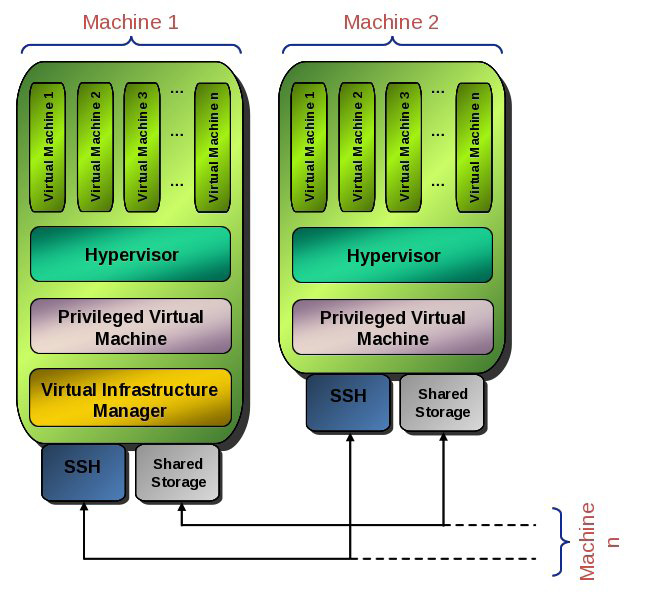
\includegraphics[scale=0.3]{resources/CloudTestBed.png}
\caption{School of Computing Cloud Testbed Architecture}
\end{figure}

\subsection{Node Specifications}
The Cloud Testbed allows the creation of Virtual Machines with fixed resources. The virtual machines are each permitted 1 virtual processor core and 1GB of memory. This allows the virtual machines to have a consistent level of performance, limiting the effect of load on the underlying hardware. The physical hardware the virtual machines execute on have Intel Xeon Quad Core processors (X3360) and 4GB of memory.

The Cloud Testbed allows for up to 10 virtual machines to be created per user. Whilst data processing software such as Hadoop has been designed to use large numbers of nodes and this cluster size may be smaller than in some real-world applications of Hadoop, significantly smaller cluster sizes are used in practice. For example, Amazon limit users of their MapReduce service to 20 nodes, and require anybody exceeding that usage to request a higher quota \cite{emrlimits}. This cluster size is consistent with previous research in the field \cite{warneke2011exploiting}.

The resources provided by the Cloud Testbed are not ideal hardware for running large scale data processing problems, which typically require large amounts of memory. Whilst this will undoubtedly impact the performance of the experiments, the environment is consistent for both Hadoop and Stratosphere, and should not affect the comparison of the tools.

\subsection{Software}
Hadoop version 2.3.0 and Stratosphere version 0.5 were installed on the cluster. At present these are the latest versions of both software packages. Stratosphere was configured to use HDFS in order to limit the effect that the file system had on the experiments. The version of Stratosphere installed was not dependent on YARN, as it was felt this would limit the effectiveness of testing scalability.

The data was loaded into HDFS before the experiments, and this was not included in runtime calculation. This limits the cost of communication overhead, as the data is already distributed across nodes appropriately, rather than data having to be transferred at the start of experiments. 

\section{Programming Language \& Frameworks}
Experiments were initially implemented in the Scala programming language \cite{scalalang}. Scala is a functional programming language with Object-Orientated support, which uses the Java Virtual Machine as a runtime environment. This allows seamless integration with existing Java libraries, such as those exposed by Stratosphere and Hadoop. As a functional language, Scala has native support for higher order functions such as map - indeed, MapReduce was originally inspired by some of the fundamental operations present in functional languages \cite{dean2008mapreduce}. This allows PACT and MapReduce jobs to be represented in a very succinct and readable manner. 

In addition to being able to call existing Java libraries, there are several `wrapper' libraries which have been developed to allow for Hadoop jobs to be written in idiomatic Scala, taking full advantage of functional features such as higher order functions. Prototypes were creating using Scalding \cite{scalding}, a library developed by Twitter, but use of this framework was later discontinued as it lacked support for later versions of Hadoop. It was replaced by Scoobi \cite{scoobi}, an open source project by NICTA.

The standard distribution of Stratosphere features a Scala API, but it was found to be too unstable for experiment development, with significant changes to the interface between different software versions. For this reason, Stratosphere experiments were reimplemented in Java, whilst reusing the core, technology agnostic processing logic which was created in Scala. 

The difference between Java and Scala is not significant in regards to processing performance. Both languages compile to Java Virtual Machine bytecode, and are therefore largely interchangeable. 
\section{Reverse Link Graph}
The Reverse Link Graph can be computed using a single Map and Reduce operation. The implementation is therefore very similar across Hadoop and Stratosphere, as it does not use any of the additional functionality present in PACT.

The Reverse Link Graph experiment was run a number of times to give an average runtime performance, as runtime can be affected by a number of external elements. 

The first step of computing the Reverse Link Graph is the Map operation. The Map stage operates on each of the documents (or articles) in the Wikipedia dataset. It extracts any HTML anchor tags from the source code of the document, and returns a list of link pairs, with the first item being the destination of the link, and the second item being the source (the current document) that the link is from.

The reduce step relies on the runtime (either Hadoop or Stratosphere) to group the items by key, so the links are grouped by the destination. The reduce step can then combine the sources into a string, giving a list of the pages which link to that destination. 

\begin{figure}[H]
\begin{tikzpicture}

% No indentation, or it'd be included on the diagram! D:

\node[doc,scale=0.5] (input) {
\begin{lstlisting}[language=html]
<html>
  <body>
    <a href="page1.htm">
      Example Article
    </a>
  </body>
</html>
\end{lstlisting}
};

\node[draw, circle, minimum size=1.5cm, right=of input] (Map) { Map };

\node[doc,scale=0.5, right=of Map] (linkpairs) {
\begin{lstlisting}
(dest1, src2)
(dest1, src3)
(dest2, src1)
(dest3, src4)
(dest3, src6)
(dest3, src7)
\end{lstlisting}
};

\node[draw, circle, minimum size=1.5cm, right=of linkpairs] (Reduce) { Reduce };

\node[doc,scale=0.5, right=of Reduce] (output) {
\begin{lstlisting}
(dest1, "src2, src3")
(dest2, "src1")
(dest3, "src4, src6, src7")
\end{lstlisting}
};

\path[->] (input) edge (Map);
\path[->] (Map) edge (linkpairs);
\path[->] (linkpairs) edge (Reduce);
\path[->] (Reduce) edge (output);

\end{tikzpicture}

\caption{A graphical representation of the Reverse Link Graph workflow}
\end{figure}

\section{PageRank}
PageRank is a more complex algorithm than the Reverse Link Graph computation, and benefits from the more advanced features of PACT. In particular as an iterative algorithm, the PageRank algorithm benefits from having iteration functionality built-in to Stratosphere. 

As Hadoop lacks some of the necessary operations to implement PageRank in an ideal way, the algorithm was implemented in twice, with the different technologies having different implementation styles. For Stratosphere, all of the features available to PACT were used, whereas with Hadoop the implementation is limited to being expressed in a MapReduce fashion.

The PageRank experiment was run a number of times to give an average runtime performance, as runtime can be affected by a number of external elements. 

For both implementations the PageRank algorithm ran for 3 iterations. This was in order to provide a fair illustration of how well iterative algorithms perform in both technologies, whilst not being prohibitively time consuming (especially on smaller cluster sizes).

\subsection{Stratosphere Implementation}
The stratosphere implementation of PageRank was the `ideal' implementation, as it has native support for a number of operations required by the PageRank algorithm. 

The first step in the process was to take the input data from the data source, and build the Reverse Link Graph. The PageRank algorithm determines the rank of a page by considering other pages which link to it, which requires the Reverse Link Graph to be computed. 

Once the Reverse Link Graph had been found, the iterative process could begin.

Each node received the PageRank of its neighbours using a Join operation, finding the scores of other nodes by their unique identifiers (the page name). The resulting data was then sent to a Reduce operation, which computed the new rank of the node by summing the rank of its neighbours, and multiplying the resulting value by a `dampening value'. 

After the first map operation, this process was applied iteratively 3 times. 

\begin{figure}[H]
\centering
\begin{tikzpicture}

% No indentation, or it'd be included on the diagram! D:
\node[circle] (dummy1) {};

\node[doc,scale=0.5, above=of dummy1] (input1) {
\begin{lstlisting}
(page1, 0.5)
\end{lstlisting}
};

\node[doc,scale=0.5, below=of dummy1] (input2) {
\begin{lstlisting}
(src1, 0.3)
(src2, 0.7)
\end{lstlisting}
};

\node[draw, circle, minimum size=1.5cm, right=of dummy1] (Join) { Join };

\node[draw, circle, minimum size=1.5cm, right=of Join] (Reduce) { Reduce };

\node[draw, right=of Reduce] (container) {

\begin{tikzpicture}
\node[rotate=90] (dots) {...};

\node (dummy2) {};

\node[doc,scale=0.5, above=of dummy2] (output1) {
\begin{lstlisting}
(page1, 0.8)
\end{lstlisting}
};

\node[doc,scale=0.5, below=of dummy2] (output2) {
\begin{lstlisting}
(src1, 0.5)
\end{lstlisting}
};

\end{tikzpicture}
};

\path[->] (input1) edge (Join);
\path[->] (input2) edge (Join);
\path[->] (Join) edge (Reduce);
\path[->] (Reduce) edge (container);
\path[arrow, dashed] (container) |- (3, 3) -| (Join);

\end{tikzpicture}

\caption{A graphical representation of the iterative part of PageRank}
\end{figure}

\subsection{Hadoop Implementation}
As Hadoop lacks the necessary operations to perform the PageRank algorithm, it must be implemented using a series of Map and Reduce operations. 

The initial process of converting the input data to the necessary format by performing the Reverse Link Graph calculation took a single Map and a Reduce operation. 

For each iteration of the algorithm, a Map and Reduce operation was required to join the node with its edges. A further MapReduce step was required to compute the updated rank for the page (as with Stratosphere). A final MapReduce step was taken to format the data in an appropriate format for the next iteration, a step taken automatically by Stratosphere.

It took a total of 10 MapReduce passes to compute the PageRank over 3 iterations.

\section{Conclusion}
This chapter has detailed the implementation concerns of the experiments. We have determined the data to be used, the runtime environment of the experiments, and the relevant data processing tool configurations. A description of the Reverse Link Graph and PageRank implementations has been given, and implementation concerns such as data format, node counts, and programming languages and frameworks used have been discussed.
\chapter{Technical Evaluation}
\section{Results Analysis}

\subsection{Hadoop Reverse Link Graph}

\subsection{Stratosphere Reverse Link Graph}

\subsection{Hadoop and Stratosphere Reverse Link Graph Comparison}

\subsection{Hadoop PageRank}

\subsection{Stratosphere PageRank}

\subsection{Hadoop and Stratosphere PageRank Comparison}

\section{Hypothesis Evaluation}

\chapter{Project Evaluation}
\centerline{\rule{149mm}{.02in}}
\vspace{2cm}

This chapter will evaluate the Final Year Project as a whole, focusing on the process, methodology and schedule of the project, and discussing its relevance to the larger research landscape.

\section{Methodology Evaluation}
Applying an Agile methodology was a key factor in successfully completing the project. The original project plan was very ambitious, and it quickly became clear that it was infeasible to complete this much work within the limited time frame of the Final Year Project. Following an Agile process was essential in prioritising the most important work, ensuring that a minimum viable amount of work was completed as quickly as possible, empirically adjusting the schedule as required throughout the project and forming contingency plans where necessary.

The methodology can be deemed successful as all of the minimum requirements were met. Minimum requirements were prioritising and carried out in earlier sprints to ensure that sufficient amount of work was completed for the project. When the higher priority minimum requirements were met, the additional goals were prioritised based on their impact to the project and carried out in priority order. 

Agile development provided a framework for adjusting the schedule throughout the project. Reviewing progress every week, and using this information to inform the next weeks estimates made the estimation process much more accurate. Previous weeks provided evidence of how long to realistically expect a task to take, helping to avoid continually overestimating the work that could be completed. 

\subsection{Schedule Adjustments}
Various adjustments were made to the schedule to ensure that the project was completed on time. Initially, the project was fairly ambitious in scope. Unfortunately, because of time constraints not all of the extended requirements could be met. Carrying work out in an iterative manner was key to the ability to remove work from the schedule (thereby ensuring the project could complete on time) whilst ensuring the minimum requirements were still met.

\todo{Change to be adjusted from modified gantt chart}
\begin{figure}[H]
\centering
\begin{ganttchart}[
	vgrid,
	hgrid,
	]{1}{16}
	\gantttitle{Project Schedule (weeks)}{16} \\
	\gantttitlelist{1,...,16}{1} \\
	\ganttgroup{Background Research}{1}{5} \\
	\ganttbar{Aims \& Objectives}{1}{1} \\
	\ganttbar{Literature Review}{2}{5} \\
	\ganttmilestone{Presentation to Distributed Systems Group}{4} \\
	\ganttbar{Experiment Prototypes}{4}{5} \\
	\ganttmilestone{Mid Project Report}{6} \\
	\ganttgroup{Experiment Implementation}{6}{13} \\
	\ganttbar{Configure Cluster}{6}{10} \\
	\ganttbar{Data Acquisition}{7}{9} \\
	\ganttbar{Reverse Link Graph Development}{8}{9} \\
	\ganttbar{PageRank Development}{10}{11} \\
	\ganttbar{Run Experiments}{11}{14} \\
	\ganttmilestone{Progress Meeting}{13} \\
	\ganttgroup{Evaluation}{13}{15} \\
	\ganttbar{Evaluation}{13}{15} \\
	\ganttbar{Report Write-up}{14}{15} \\
	\ganttbar{Proof Reading \& Adjustments}{16}{16} \\
	\ganttmilestone{Deadline}{16}
\end{ganttchart}
\caption{Final Gantt Chart of Project Schedule}
\label{endGantt}
\end{figure}

In comparison to the initial project estimation, setting up the cluster of machines took much longer than expected. It was expected that Hadoop and Stratosphere would be pre-installed on the Cloud Testbed, but this was not the case for Stratosphere, and Hadoop had an outdated version. The process of installing and configuring the software took longer than expected, leading to the cluster set-up to take 4 weeks, rather than the week originally predicted.

In order to compensate for this, the data required for the experiments was acquired and pre-processed as the cluster was being configured. As stages in these tasks were passive (e.g. waiting for large amounts of data to download) these tasks could be performed in parallel efficiently. 

Rather than performing the experiments required for the minimum requirements (e.g. Word Count or Terasort), more complex experiments were developed to better reflect the real-world usage of the data processing tools. This met an additional requirement (in addition to the minimum requirements). Implementing the more complex experiments directly and not performing the basic experiments was a more efficient use of time, with more value being gained from the advanced experiments, and time not being spent on performing the simpler experiments. 

Experiments could be run in parallel to the evaluation and write-up stages, as experiments (particularly Hadoop PageRank) often took a large amount of time to finish without requiring any supervision. This left time to write up various aspects of the report, and evaluate experiments which had already been completed (for example, evaluating the results of the Reverse Link Graph experiments as PageRank was running).

The project was completed slightly ahead of schedule, allowing for a week of proof reading and adjustments to the report.

\section{Achievement of Aims \& Objectives}
The stated aim of the project was to provide a reasoned and objective analysis of the efficiency of Hadoop and Stratosphere. This aim was met through meeting the following requirements.

\subsection{Minimum Requirements}
\begin{itemize}
	\item Install Hadoop
	\todo{More?}
	Hadoop was installed on the Cloud Testbed.

	\item Install Stratosphere
	\todo{More here too?}
	Stratosphere was installed on the Cloud Testbed.

	\item Run a MapReduce processing task

	In the original requirements, example exercises such as Word Counting and Terassort were discussed as potential MapReduce problems which could be used to benchmark Hadoop and Stratosphere. This requirement was met by running the Reverse Link Graph experiment on both tools. This will be discussed further in the `Real-world problem' extended requirement.

	\item Run a non-MapReduce processing task

	In the original requirements, K-Means clustering was discussed as a problem which could be used to compared the ability of Stratosphere and Hadoop to run problems that do not conventionally fit in to the MapReduce paradigm. This requirement was met by calculating the PageRank of the data. PageRank is an experiment included in both Hadoop libraries, and as an example in the standard distribution of Stratosphere. The code for both of these had to be modified to meet the input format.

	\item Run an experiment on a different cluster size

	This requirement was met, as all experiments were executed on various different cluster sizes.
\end{itemize}

\subsection{Extended Requirements}
\begin{itemize}
	\item Real-world problem

	In the original requirements the use of a `real-world' problem was discussed as it would provide a less artificial way of evaluating Hadoop and Stratosphere. It was not possible to identify a suitable problem for various reasons. The availability and size of data were a limiting factor, as was finding an experiment with sufficient literature which did not require extensive domain specific knowledge. Due to the time constraints of the Final Year Project, it was deemed infeasible to complete a dedicated real-world problem.

	Rather than running the real-world problem as a separate experiment, it was decided that the MapReduce and non-MapReduce problems should be chosen in such a way that they reflected many of the properties present in real-world scenarios. The Reverse Link Graph has various real-world applications and PageRank forms a core part of search engine technology. The PageRank experiment required code to be modified to match the input data, where the Reverse Link Graph experiment was developed from scratch.

	Whilst the requirement may not have been met directly, the fundamental ideas behind the extension have been met, and the value toward the project has therefore been achieved.

	\item Scale all experiments

	All experiments have been run on various different cluster sizes. In addition to this, rather than simply running them on 2 different cluster sizes, each has been executed on cluster sizes of 2, 4, 6, 8 and 10 machines. This extended requirement has been met. 

	The only exception to this is the PageRank algorithm on Hadoop. This was only run on 6, 8 and 10 nodes as resource constraints prevented it from working on 2 and 4 nodes. 

	\item Public Cloud

	Unfortunately the experiments were not completed on a public cloud. It was felt that this extended requirement had the lowest priority, as it would have a limited effect on the results of the experiments and required a significant investment of time and money. Running the same experiments on a different cloud would likely replicate the results, which provides limited value in the context of the experiment. Two areas which may have benefited from using a public cloud would be that experiments could have been run on a larger scale (for example, 16 nodes to continue the scalability experiments, or using larger data) and the resource acquisition technique of Stratosphere could have been evaluated. This has been identified as an area of potential future research.
\end{itemize}

\section{Related Work}
A key part of evaluating the project is viewing the research in the context of previous work in the field.

\subsection{Comparison to Prior Work}
Specifically, there are two core Nephele papers which have previously studied the performance characteristics of Stratosphere (then Nephele) by comparing it to Hadoop (``Exploiting Dynamic Resource Allocation for Efficient Parallel Data Processing in the Cloud'' \cite{warneke2011exploiting} and ``Nephele/PACTs: a programming model and execution framework for web-scale analytical processing'' \cite{battre2010socc}). 

The experiments carried out in this project support the performance findings of the previous work, finding that Stratosphere outperforms Hadoop in cases of both MapReduce and non-MapReduce problems, with MapReduce being particularly poor when considering iterative problems.

\todo{Table of comparison (here or in contribution?)}

\subsubsection{Contribution to Research}
The work carried out in this project is intended to contribute to the existing landscape by building on the work of previous research. This project attempts to contribute to the existing body of research in the following ways

\begin{enumerate}
	\item Performing experiments designed to test the scalability of tools, and how they react to changing resources. The existing research typically uses one fixed size cluster, with some prior research focusing on a comparison between a fixed Hadoop cluster and a Stratosphere cluster using automated resource acquisition. In this project, experiments have been run across varying cluster sizes, allowing a discussion of how well the tools respond to changing resources (in the form of cluster size).
	\item The experiments have been chosen to be non-trivial in nature. This is in contrast with many existing benchmarks, which use synthetic tasks (such as Word Counting or Terasort) and data created for the sole purpose of experimentation. By comparison, we have chosen problems which attempt to reflect the real-world usage of data processing tools, with existing data sources used for experimentation. 
	\item By providing a performance comparison and replicating the results of prior research using later versions of Hadoop and Stratosphere. This is significant as the existing performance comparisons use earlier versions of software, and since this point the Stratosphere project in particular has changed significantly (becoming an Open Source project and being accepted on to the Google Summer of Code and Apache Incubator projects).
\end{enumerate}

\subsection{Future Work}
\todo{Bullet Points!}
There are a number of possible extensions to the project which could be tackled as future work.

A particular area which was identified as an extended goal of the project was to look at the performance of the data processing tools in a public cloud environment. In particular, this work could look at the impact of the unique method in which Stratosphere can acquire resources rather than processing data on a fixed cluster size, and how this approach effects performance and scalability. The cost of public clouds, and whether the choice of data processing tool can reduce cost could also be an area of research.

Various cloud providers offer hosted Platform as a Service data processing tools (typically Hadoop) which allow users to process data without worrying about manually configuring a cluster. A possible extension to this work would be to consider how this effects the performance of data processing tasks, and whether the elasticity afforded by a Platform of a Service approach is appropriate for data processing scenarios. 

An alternative direction would be to look at other, more specialised data processing tools which are designed to process certain types of data (for example, large scale graph processing tools). 

\todo{Full conclusion chapter}
\chapter{Project Conclusion}
\centerline{\rule{149mm}{.02in}}
\vspace{2cm}

The aim of this project was to carry out a objective performance analysis of the tools available for processing large amounts of data in parallel. Specifically the current standard data processing technology (the Hadoop implementation of the MapReduce paradigm) was compared with a newer, more research led effort (the Stratosphere implementation of the PACT programming paradigm). At the beginning of the project, three research goals were identified to meet this aim.

\begin{itemize}
	\item Does PACT overcome the inherent disadvantages of the MapReduce paradigm?
	\item How well does Stratosphere perform MapReduce tasks?
	\item How do Hadoop and Stratosphere perform in a highly elastic Cloud Computing environment?
\end{itemize}  

The research goals were met by deriving a series of experiments. 

In order to determine how well PACT overcomes the inherent disadvantages of MapReduce, both tools calculated the PageRank of a set of Wikipedia articles. This tested the ability of the tools to perform iterative algorithms (a known issue with the MapReduce paradigm), and to perform multiple operations per iteration (joining the data and then computing the PageRank). 

The second experiment determined how well Stratosphere could perform MapReduce tasks, by finding the Reverse Link Graph of a set of Wikipedia articles. This is a problem naturally applicable to MapReduce and therefore well suited to Hadoop.

Finally, each experiment was executed on a number of different cluster sizes, and the results compared to determine the scalability of each of the systems.

The results of the first two experiments overwhelmingly showed that Stratosphere performed better than Hadoop in cases where a task can be simply formulated as a MapReduce problem, and those where it cannot. In particular, there are significant performance enhancements in iterative scenarios.

The experiments also determined that both tools scale in a near-linear fashion. 

These results are replicated in previous work in the research area. This project has contributed to the existing research by running novel problems, analysing the scalability of the tools, and replicating results on up-to-date versions of the software. 

\addcontentsline{toc}{chapter}{\numberline { }Bibliography}
\bibliographystyle{plain}
\bibliography{refs}      % include the bibliography

\appendix                % include the appendices
\chapter{Personal Reflection}
\centerline{\rule{149mm}{.02in}}
\vspace{2cm}

At the beginning of my degree I found it difficult to imagine dedicating such a large amount of time to one topic. 

I feel one of the key factors in finishing the project successfully was following an Agile approach. Reviewing the work completed on a weekly basis helped make more realistic estimates for future work, and let to more realistic scheduling. In order to facilitate this, I'd recommend other students to provide a relatively loose schedule in the early stages of the project. It is likely that the (feasible) requirements for the project will become more clear as the project progresses, and having a flexible schedule allows for changes as things become clearer. Having a loose schedule also allows for adjustments when things go wrong. Inevitably tasks will take longer than expected and work will appear which was not anticipated. 

The Final Year Project provides very strict milestones in terms of the deadlines imposed on students. My experiment design was modular in nature, so certain experiments could be cut or simplified when there was not enough time to implement the original plan. The ability to cut scope whilst still meeting the minimum requirements is essential in a project of this nature, with very strict, immovable deadlines. 

Maintaining this methodology relies on the student having discipline to set clear goals each `sprint', and to review the progress towards those goals at the end in order to accurately ascertain what amount of work is feasible for each time period. For the Final Year Project I found that a week was naturally suited to being the length of a sprint, as supervisor meetings provided an opportunity to reflect on progress and set goals. It is much easier to set realistic expectations in the short term, rather than over the length of the whole project.

Taking the time to set out a strong set of Aims \& Objectives at the beginning of the project was something which served me well, as it provided a clear end goal for the project. While the method of getting there changed, having a core direction to aim toward was helpful.

From a technical perspective I would encourage students undertaking Big Data projects to be wary of the length of time it takes to correctly configure Hadoop and similar tools. They are far more complex than they initially appear; this was the cause of the largest deviation from my project schedule. Similarly, I found several problems with libraries and frameworks. In particular, working with a beta version of Stratosphere caused significant problems at points. I would encourage future students to work on stable branches of software whenever possible, and to strongly consider whether the move to a less stable version is worth the additional features.

Using version control helped greatly throughout the project, allowing me to experiment with the experiment code without worrying about losing any prior, working code. It also made it much simpler to work on any machine, and ensured that the project was well backed up throughout. 

I would strongly encourage future students to take a project in an area of interest, and to choose a topic which will challenge them. The Final Year Project provides an excellent opportunity to learn new topics and work in interesting areas in much more depth than the rest of the degree program.
\chapter{Record of External Materials Used}
\centerline{\rule{149mm}{.02in}}
\vspace{2cm}

\begin{itemize}
	\item Data was acquired from the Wikimedia Foundation, who provide semi-reguar HTML dumps of various language versions of wikipedia \cite{wikiDumps}, under the Creative Commons license.
	\item Software developed for the Hadoop platform used the Scoobi \cite{scoobi}, a library developed by NICTA.
	\item The Hadoop PageRank implementation was modified from code examples provided by the Scoobi \cite{scoobi} project.
	\item The Stratosphere PageRank implementation was modified from code examples provided by the Stratosphere project.
\end{itemize}
\chapter{Potential Ethical Issues}
\centerline{\rule{149mm}{.02in}}
\vspace{2cm}

No ethical issues arose during my project.



\end{document}
